\documentclass[conference]{IEEEtran}

\ifCLASSINFOpdf

\else

\fi

% correct bad hyphenation here
\hyphenation{op-tical net-works semi-conduc-tor}
\usepackage{graphicx}
\usepackage{cite}
\usepackage[usenames,dvipsnames]{color}
\usepackage{hyperref}
\usepackage{amsmath}
\usepackage{amsfonts}
\usepackage{amssymb}
\usepackage{makeidx}
\usepackage{graphicx}
\usepackage{lmodern}
\usepackage{kpfonts}
\usepackage[usenames,dvipsnames]{color}
\usepackage[left=2cm,right=2cm,top=2cm,bottom=2cm]{geometry}
\usepackage[dutch]{babel}
\usepackage{listings}

\begin{document}

\title{Totem Health Patch\\Embedded System Guide}

% author names and affiliations
% use a multiple column layout for up to three different
% affiliations
\author{\IEEEauthorblockN{Totem Open Health}
\IEEEauthorblockA{Product: Totem Health Patch\\
Versie: 1\\
Datum: 15-02-2016\\
Handleiding voor gebruik 'Totem Health Patch'}}

\maketitle

\begin{center}
    
\includegraphics[scale=0.9]{logototem}
    \begin{minipage}{0.6\textwidth}
    \footnotesize
    \emph{Totem logo}
    \end{minipage}
\end{center}

\begin{abstract}
Totem is de drijfveer achter de Totem Health Patch. Een opensource smart object die uiterst geschikt is voor medisch onderzoek, educatieve doeleinden of voor de hobbyprogrammeur. In dit document wordt de installatie en werking van de Totem Health Patch uitgelegd. Vragen zoals: 'wat is de Totem Health Patch precies?', 'wat heb ik nodig om de Totem Health Patch werkend te krijgen met de meest recente voorbeeldprogramma's? en 'wat zijn belangrijke zaken waarop gelet moet worden tijdens de installatie?'. Naast de installatie wordt de Totem Health Patch Android applicatie en firmware versie 1 uitgelegd.   
\end{abstract}

\IEEEpeerreviewmaketitle

\section{Introductie}
Met de open source wereld is vrijwel alles mogelijk. Men zegt vaak  'je bent pas echt de eigenaar van een product, wanneer het open source is'. Niet alleen de software van de Totem Health Patch is open source, maar ook de hardware. Dit maakt de Totem Health Patch aantrekkelijk voor zowel de educatieve wereld als de zorgsector. De Totem Health Patch is een draagbaar systeem met alle nodige sensoren aan boord. Met een accelerometer, gyroscoop, temperatuursensor, bluetooth module en SD kaart lezer/schrijver, is de gebruiker in staat om een analyse te schetsen van lichamelijke omstandigheden. Zo kan handige data bijvoorbeeld opgeslagen worden op een SD kaart en later worden ontleed voor statistische onderzoeken. In dit document wordt laten zien hoe de Totem Health Patch in enkele stappen al kan functioneren als smart meetobject.\\\\\\\\\\\\\\\\\\\\\\\\   

\section{Benodigdheden}
Wat is nodig om de Totem Heath Patch te programmeren en te gebruiken.\\\\-Totem Heath Patch\\
-Internet toegang\\
-Totem Programmeer Rig\\
-J-link programmeer module\\

\section{Gereed maken voor programmeren}
De Totem Health Patch wordt geprogrammeerd met een J-Link programmeer module. De programmeer module programmeert de gecompileerde .hex bestand in de NRF51822 chip. Het .hex bestand wordt gegenereerd door de mbed web-compiler. Mbed is tevens ook de ontwikkelomgeving voor de Totem Health Patch. Stap voor stap wordt uitgelegd hoe de Totem Health Patch geprogrammeerd moet worden met zelfgemaakte firmware of voorbeeld firmware.

\subsection{Mbed}
Klik op de onderstaande link om naar de mbed ontwikkelomgeving te gaan.\\\\\url{https://developer.mbed.org/account/login/?next=/}\\\\Maak een mbed account aan of log in met de juiste gebruikersgegevens. Druk op compiler voor de ontwikkelomgeving.
 
\begin{center}
    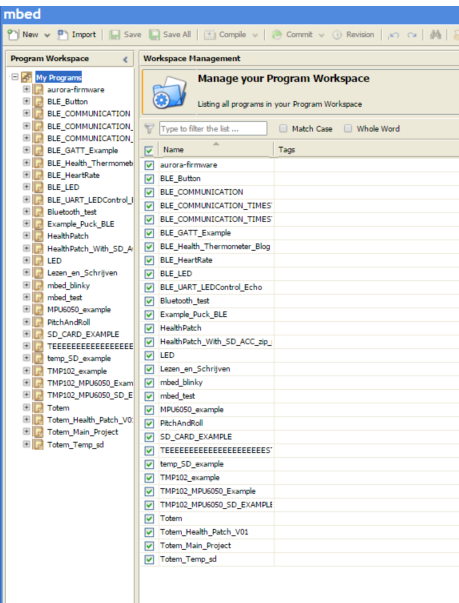
\includegraphics[scale=.8]{mbed1}
    \begin{minipage}{0.6\textwidth}
    \footnotesize
    \emph{Mbed ontwikkel omgeving}
    \end{minipage}
\end{center}

\subsection{Installatie benodigde software}
Met nRFgo Studio wordt firmware in de Totem Heath Patch geprogrammeerd. Voer een schone installatie uit, door op de volgende link te drukken. Op deze pagina is de 64 bit versie beschikbaar voor microsoft windows. \\\\\url{https://www.nordicsemi.com/kor/nordic/Products/nRFgo-Studio/nRFgo-Studio-Win64/14964}\\\\Om een gegenereerd .hex bestand naar de Jlink programmer te sturen, moet een aparte driver worden geïnstalleerd. Met de onderstaande link kan de nieuwste Jlink driver worden geïnstalleerd.\\\\\url{https://www.segger.com/jlink-software.html}\\\\
De softwarematige onderdelen staan klaar voor het programmeren.

\subsection{Installeren programmeer Rig}
De programmeer Rig is het programmeer docking voor de Totem Health Patch. De Totem Health Patch kan gemakkelijk uit de behuizing gehaald worden, om vervolgens geprogrammeerd te worden met willekeurige firmware. De Rig is een handige tool om de Health Patch snel te programmeren zonder deze te solderen aan een programmeer module. Daarnaast is het snel testen van software makkelijk.

\begin{center}
    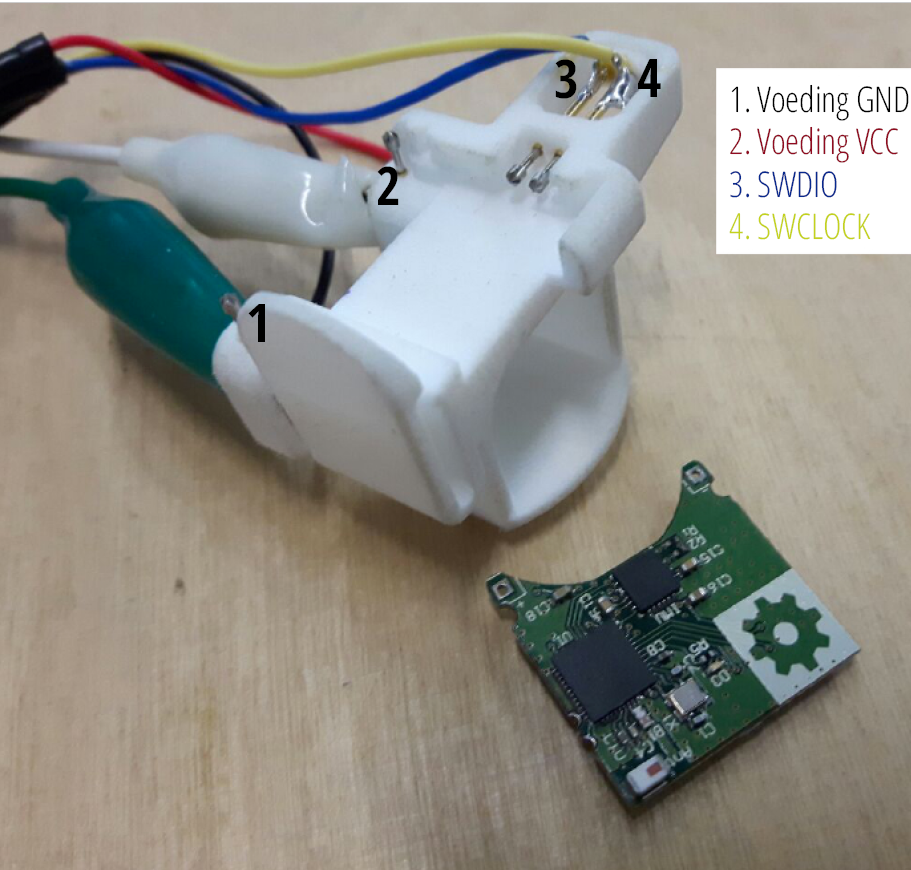
\includegraphics[scale=0.45]{rig1}
    \begin{minipage}{0.6\textwidth}
    \footnotesize
    \emph{Bekabeling programmeer Rig}
    \end{minipage}
\end{center}

De Rig heeft vier connectie punten. Twee zijn bedoeld voor voor het refereren van de spanning. Let op: tijdens het programmeren moet de batterij aangesloten zijn. De programmeer module dient niet als voedingsbron voor de Totem Health Patch. Er kan dus niet geprogrammeerd worden wanneer de knoopcel batterij niet in de batterijhouder zit. Op de volgende twee afbeeldingen wordt duidelijk hoe de programmeer Rig aangesloten moet worden op de JLink hardware.

\begin{center}
    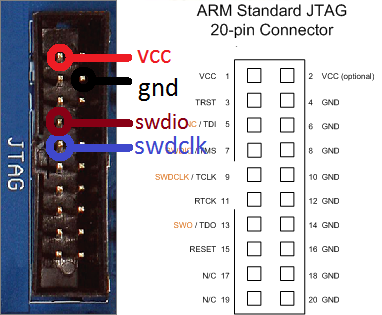
\includegraphics[scale=1.2]{jlink}
    \begin{minipage}{0.6\textwidth}
    \footnotesize
    \emph{Bekabeling JLink programmeer module}
    \end{minipage}
\end{center}

\newpage

Wanneer de hardware correct is aangesloten en de Health Patch op de juiste manier in de Rig is gemonteerd, zal de JLink programmeer module een groene indicatie geven. In nrfGoStudio is het nu mogelijk om de nRF5x Programming tab te openen. Het Segger ID is nu zichtbaar en de MCU kan geprogrammeerd worden.

\begin{center}
    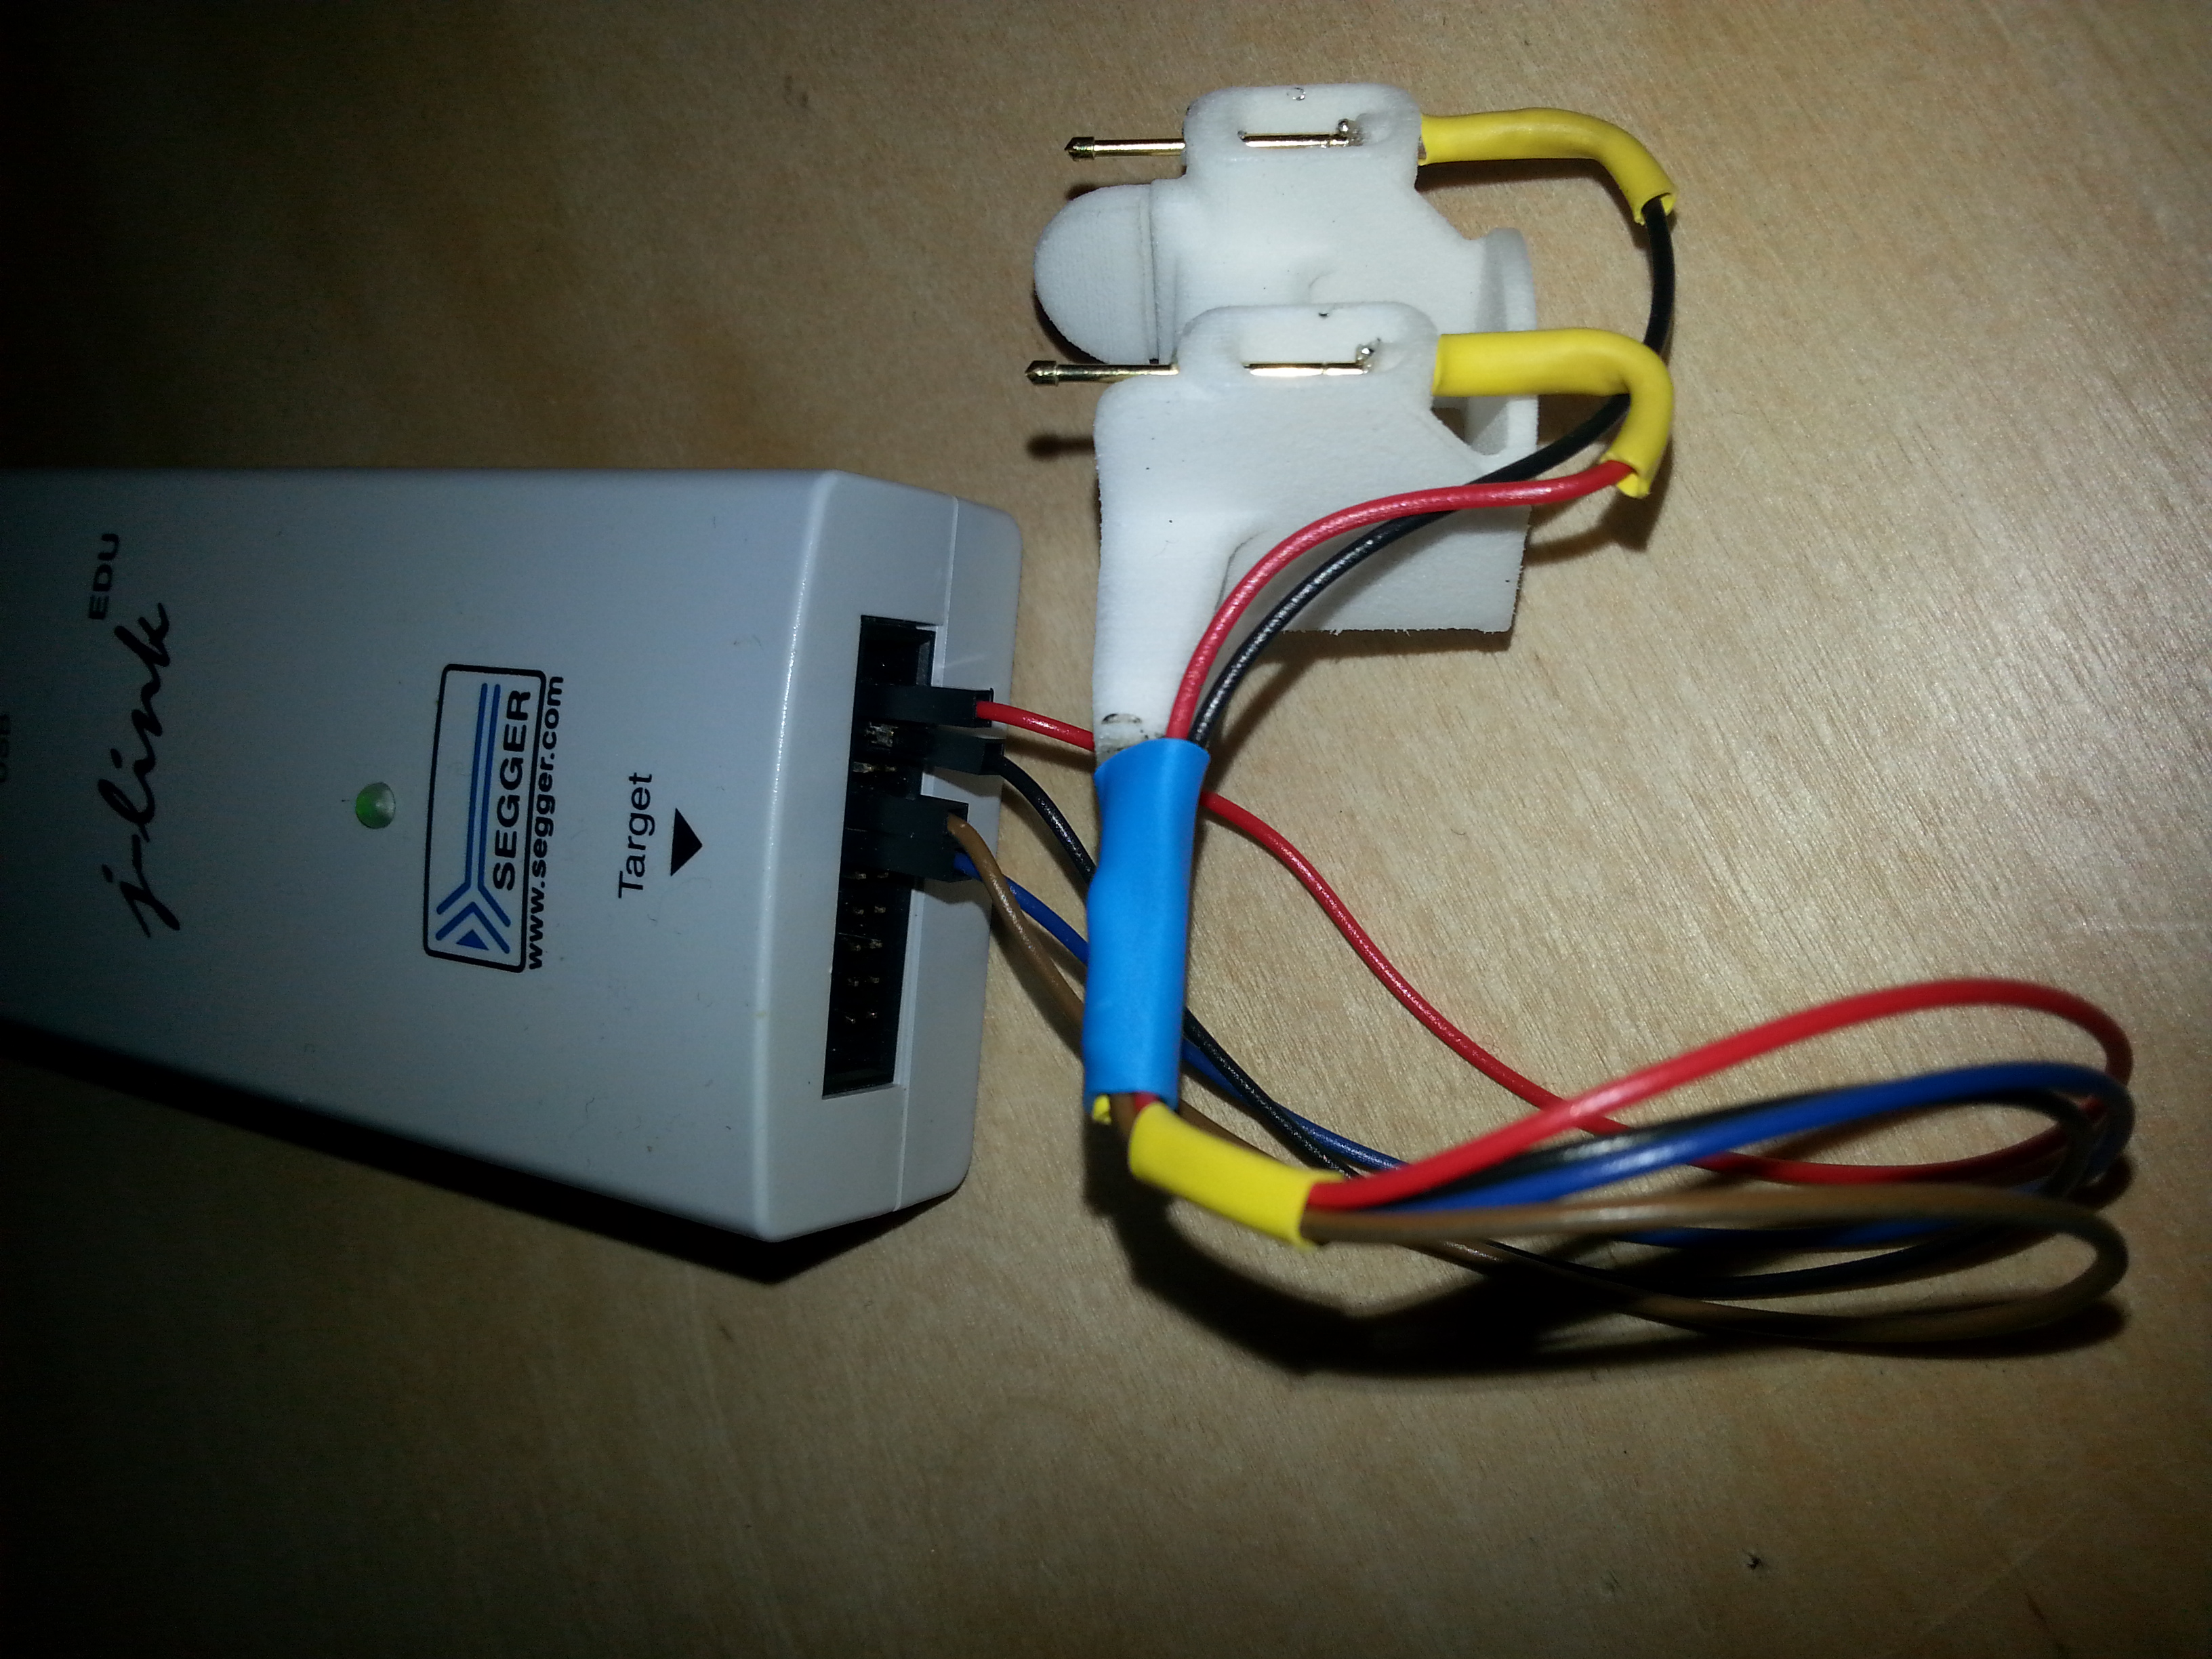
\includegraphics[scale=0.07]{jlink2}
    \begin{minipage}{0.6\textwidth}
    \footnotesize
    \emph{Overzicht JLink programmeer module}
    \end{minipage}
\end{center}

\section{Programmeren}
\subsection{Programmeren met j-link}
In de Embed software ontwikkelomgeving wordt code gecompileerd tot .hex file. De web applicatie maakt snel duidelijk dat er een specifiek type programmeer module moet worden geselecteerd. Rechts boven in de hoek van de webpagina is zichtbaar voor welk type MCU er wordt geprogrammeerd. Deze moet voor de Totem Health Patch altijd ingesteld zijn op de Nordic NRF51822 MCU. Zie onderstaande afbeelding.

\begin{center}
    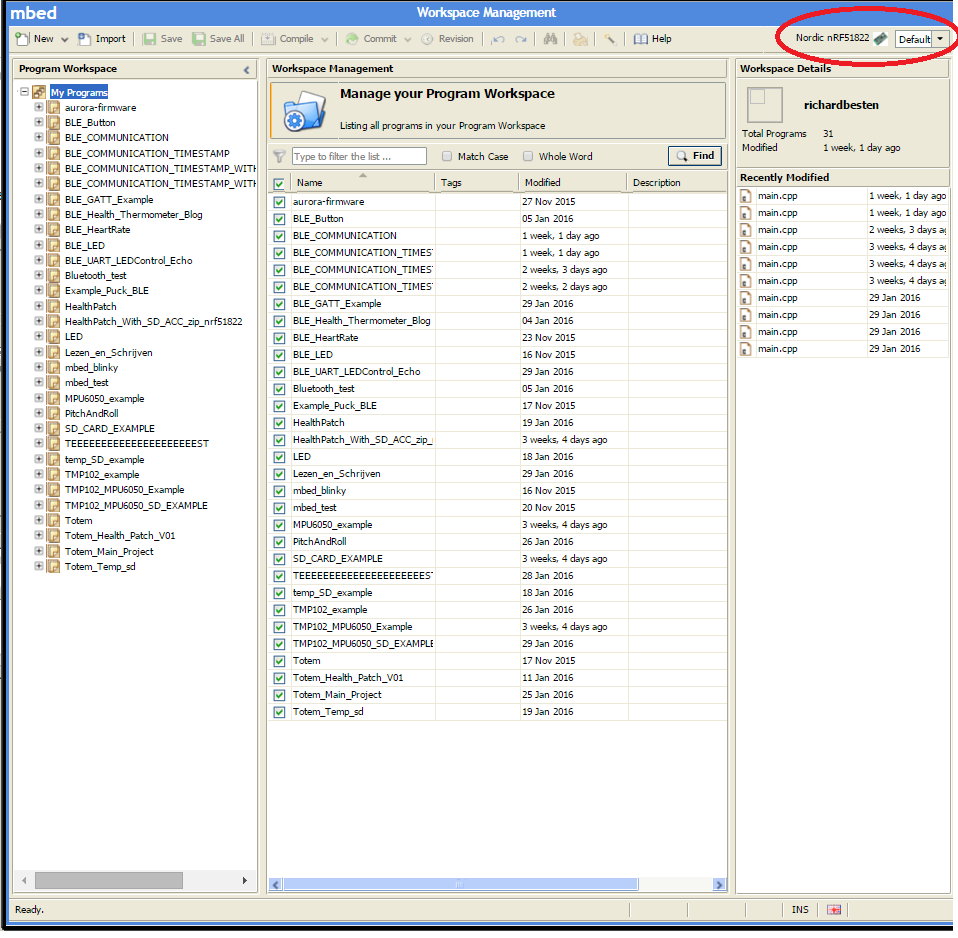
\includegraphics[scale=0.4]{mbed2}
    \begin{minipage}{0.6\textwidth}
    \footnotesize
    \emph{Nordic MPU selecteren}
    \end{minipage}
\end{center}

Er kan nu geprogrammeerd worden in de Mbed web applicatie met de juiste instellingen. Met de knop NEW -- NEW PROGRAM kan gemakkelijk een bestaand programma of nieuw programma worden geopend. Daarnaast kan er gekozen worden om een geheel extern programma in Mbed te laden. Ga naar GitHub voor de Totem Open Health software community.\\\\\url{https://github.com/wemaketotem}\\\\Hier zijn verschillende voorbeelden te vinden die speciaal ontworpen zijn voor de Totem Health Patch. Wanneer de software tot resultaat is gekomen, kan de software worden gecompileerd. De gecompileerde code wordt automatisch gedownload door de internet browser. De gegenereerde .hex file kan vervolgens worden geopend door nrfGoStudio.\\\\Het is belangrijk om het geheugen van de MCU leeg te maken, voordat de MCU geprogrammeerd wordt. Wanneer het totale geheugenlimiet niet beschikbaar is, is het niet mogelijk om nieuwe firmware in de MCU te laden. Het totale programmeer geheugen is 256kB. Na het leeg maken van het geheugen kan de firmware ingeladen worden. De firmware wordt gekozen met de knop 'Browse...'. Vervolgens wordt er op de 'program' knop gedrukt om de software daadwerkelijk in de MCU te laden. Zie voorbeeld afbeelding.

\begin{center}
    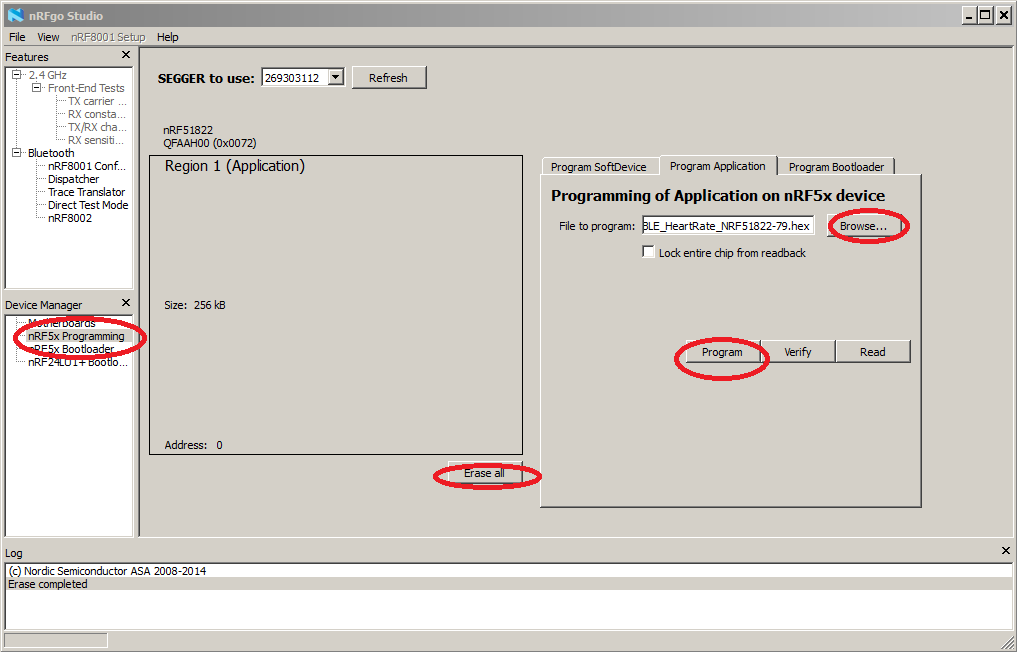
\includegraphics[scale=0.4]{gostudio}
    \begin{minipage}{0.6\textwidth}
    \footnotesize
    \emph{nrfGoStudio device programming}
    \end{minipage}
\end{center}

\subsection{Programmeren over Bluetooth}
Naast het programmeren met de j-link programmeer module is het ook mogelijk om de Totem Health Patch te flashen via bluetooth. Dit vergt een kleine voorbereiding. Hiervoor is een andere bootloader benodigd. Dit is de zogenaamde FOTA bootloader en is te vinden op de GitHub pagina van 'WeMakeTotem'. Zie onderstaande link.\\\\\url{https://github.com/wemaketotem/BLUETOOTH_AIR_FLASHING_BOOTLOADER 
}\\\\De FOTA bootloader wordt op dezelfde manier geprogrammeerd als bovenstaande instructies. Door middel van nRFgo Studio wordt de .hex file in de Health Patch geprogrammeerd. De FOTA bootloader maakt het mogelijk om via bluetooth de Health Patch te programmeren.\\\\Het is noodzakelijk om de 'nRF Master Control Panel' applicatie te downloaden via een Applicatiewinkel. Deze applicatie maakt het mogelijk gecompileerde code door middel van Bluetooth in de Health Patch te programmeren.\\\\Met de tweede stap wordt de mbed ontwikkelomgeving juist ingesteld om gecompileerde code FOTA compatible te maken. In de mbed ontwikkelomgeving moet een FOTA device geselecteerd worden. Dit is het 'Nordic nRF51822 FOTA' device platform. Dit device platform moet geselecteerd zijn om FOTA compatible firmware te genereren. Zie foto hieronder voor juiste platform selectie.

\begin{center}
    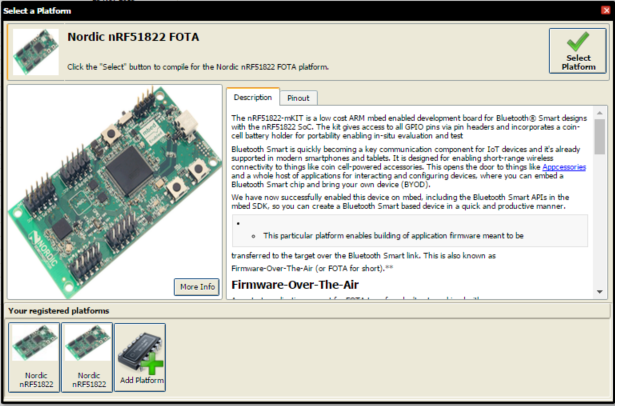
\includegraphics[scale=0.65]{FOTA0}
    \begin{minipage}{0.6\textwidth}
    \footnotesize
    \emph{FOTA device selectie}
    \end{minipage}
\end{center}

Wanneer de juiste bootloader is geprogrammeerd, is de Totem Health Patch zichtbaar in de Master Control applicatie. De Totem Health Patch is zichtbaar als 'DefaultApp'. Met connect wordt er verbinding gemaakt met het device.

\begin{center}
    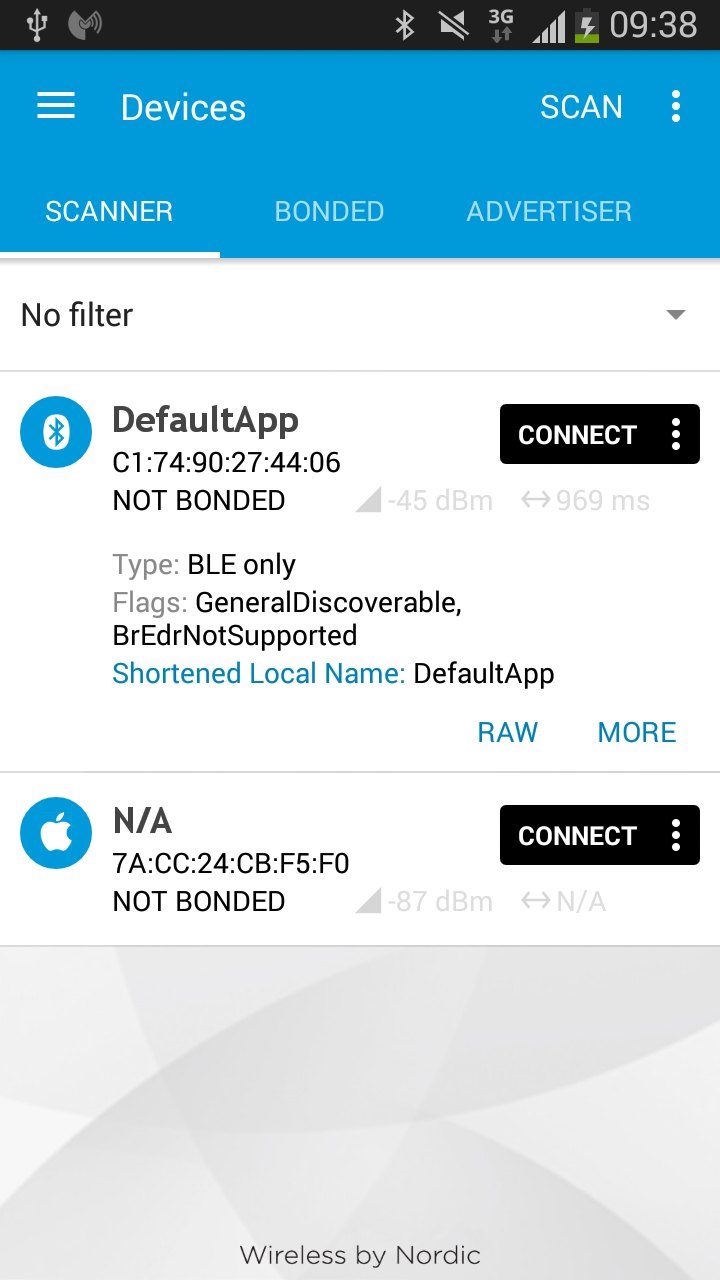
\includegraphics[scale=0.3]{FOTA1}
    \begin{minipage}{0.6\textwidth}
    \footnotesize
    \emph{DefaultApp}
    \end{minipage}
\end{center}
\newpage
Na het verbinden met de DefaultApp kan de Totem Health Patch in DFU mode gebracht worden. Om de DFU te starten moet de 'Device Firmware Udate Service' gestart worden. Door middel van het write commando in de 'DFU Control Point' service te selecteren kan er een keuze gemaakt worden tussen verschillende uplode masks. Selecteer 'Application' en druk op send om de DFU te starten. 

\begin{center}
    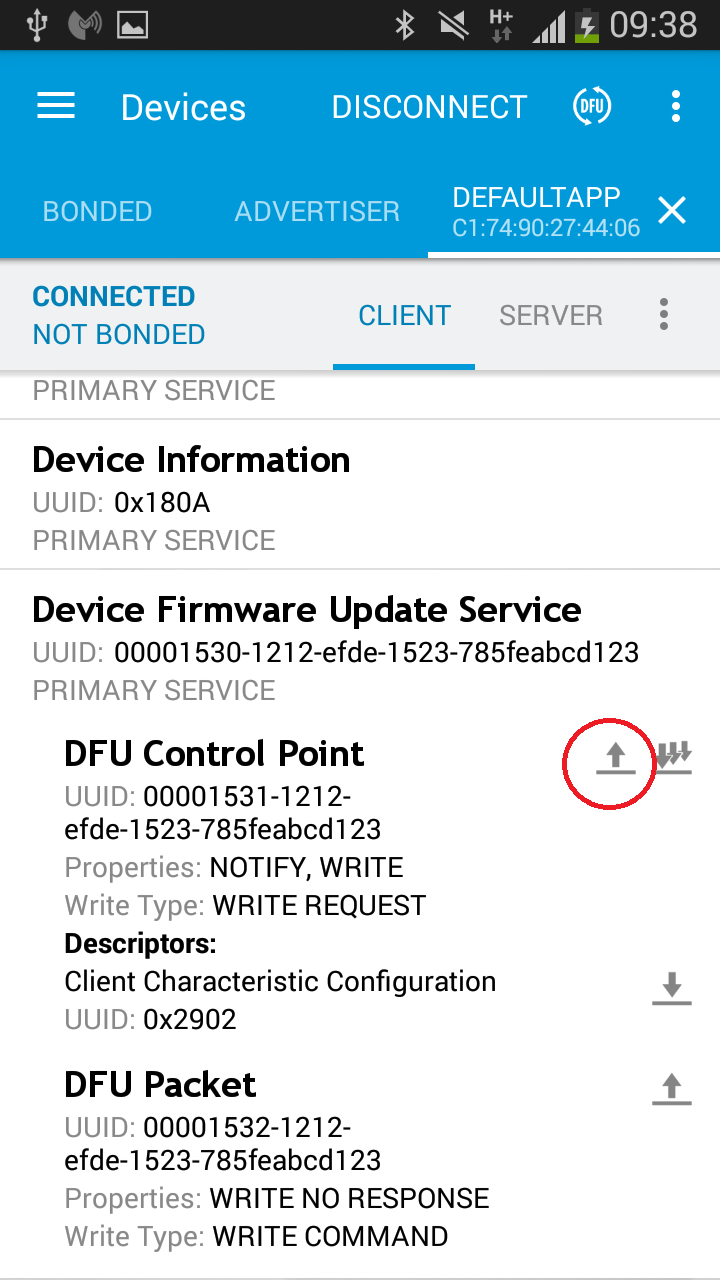
\includegraphics[scale=0.5]{FOTA2}
    \begin{minipage}{0.6\textwidth}
    \footnotesize
    \emph{Update Service}
    \end{minipage}
\end{center}

\begin{center}
    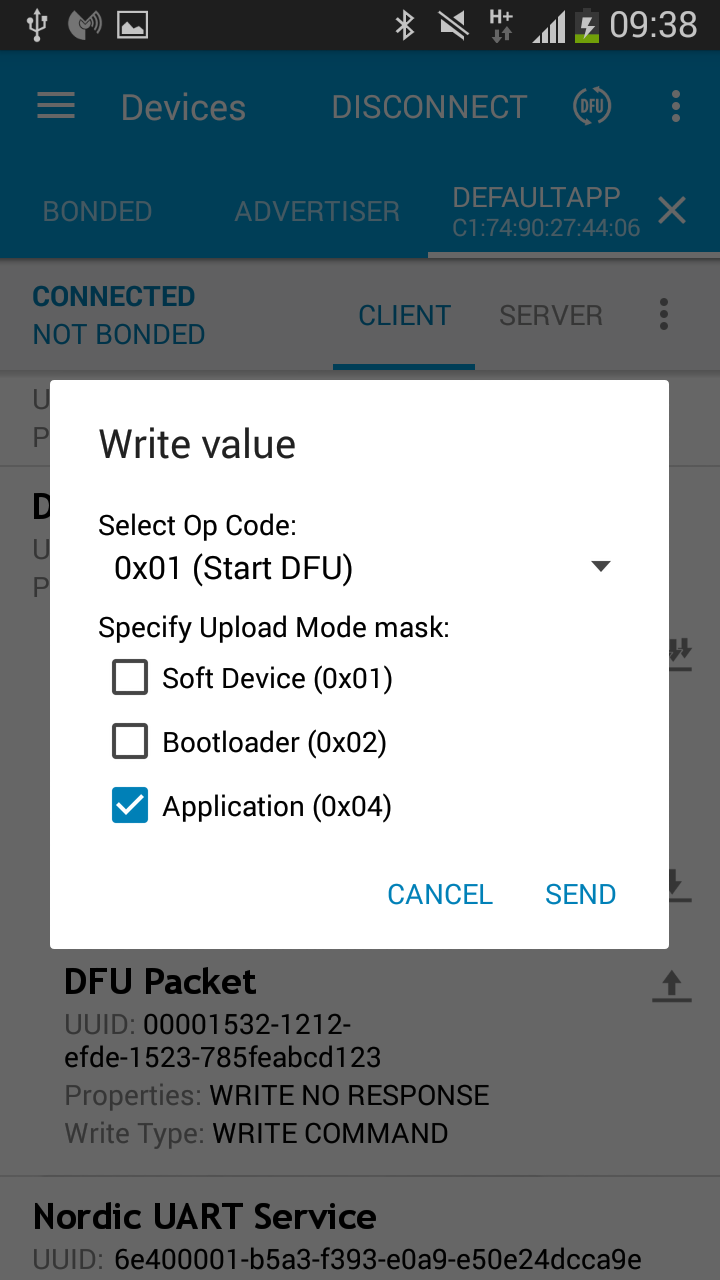
\includegraphics[scale=0.3]{FOTA3}
    \begin{minipage}{0.6\textwidth}
    \footnotesize
    \emph{Dfu Target}
    \end{minipage}
\end{center}
\newpage
Sluit de huidige verbinding af en zoek naar nieuwe apparaten om verbinding te maken met de DFU service. De Totem Health Patch is nu zichtbaar onder de naam 'DfuTarg'. Verbind de applicatie met de DFU target device. Wanneer er verbinding is gemaakt met de DFU target, is het mogelijk om firmware te selecteren. Dit is NRF51822 OTA firmware die gecompileerd is door de mbed ontwikkelomgeving.  

\begin{center}
    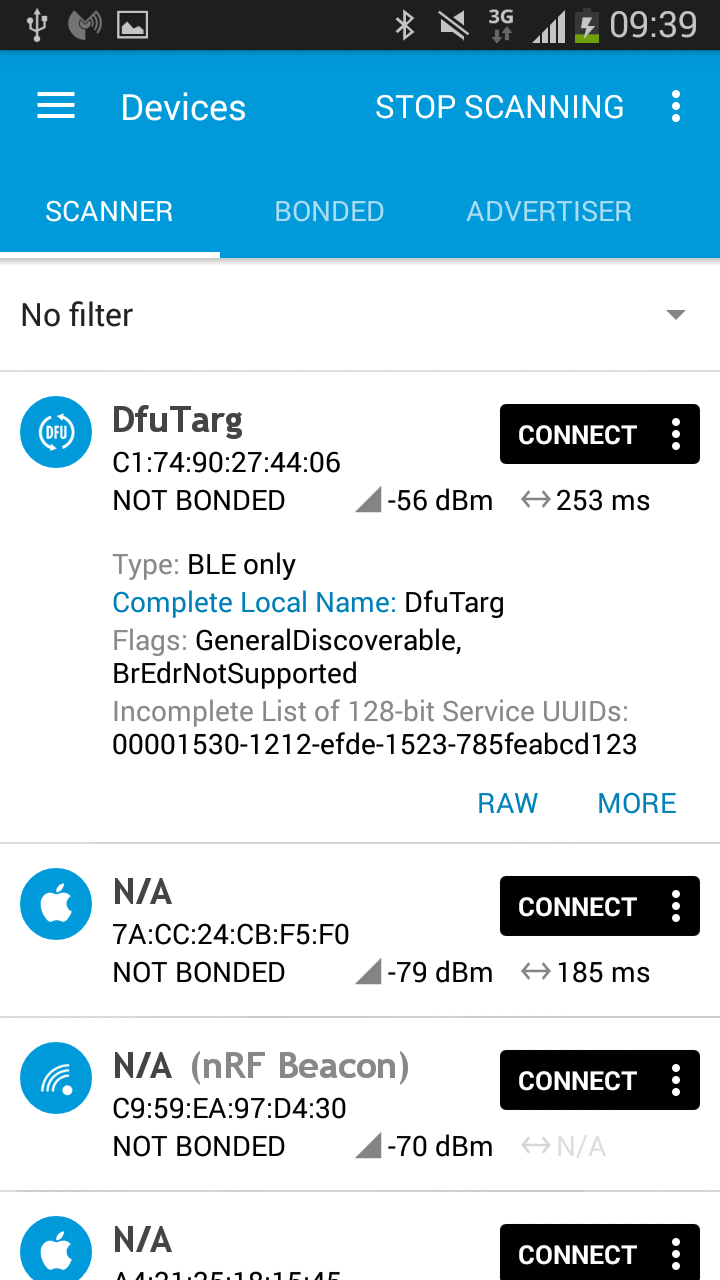
\includegraphics[scale=0.3]{FOTA4}
    \begin{minipage}{0.6\textwidth}
    \footnotesize
    \emph{Dfu Target select}
    \end{minipage}
\end{center}

Rechts boven in de hoek van het DFUTARG device is een klein icoontje zichtbaar, waarmee de firmware geselecteerd kan worden. Opnieuw kan nu gekozen worden welk type file er geupload moet worden. Voor gecompileerde firmware moet 'Application' afgevinkt worden. Met het OK commando wordt de file selector geactiveerd. 

\begin{center}
    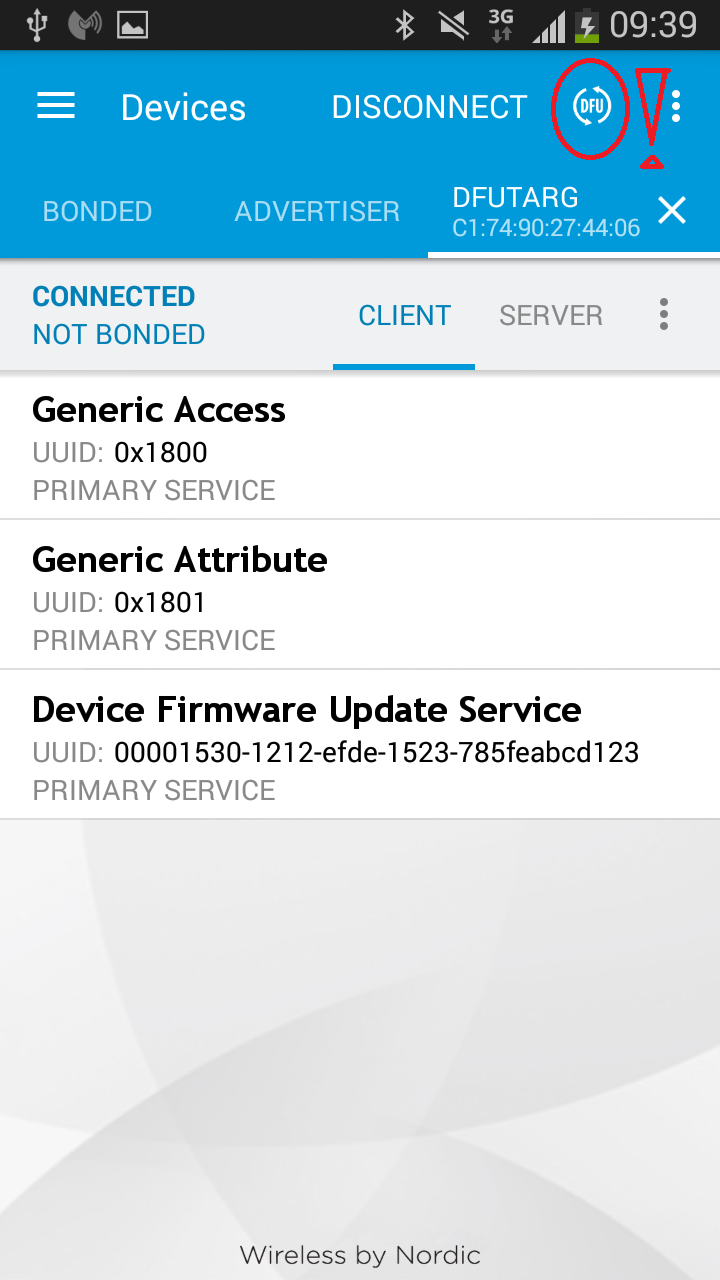
\includegraphics[scale=0.5]{FOTA5}
    \begin{minipage}{0.6\textwidth}
    \footnotesize
    \emph{Select DFU}
    \end{minipage}
\end{center}

\begin{center}
    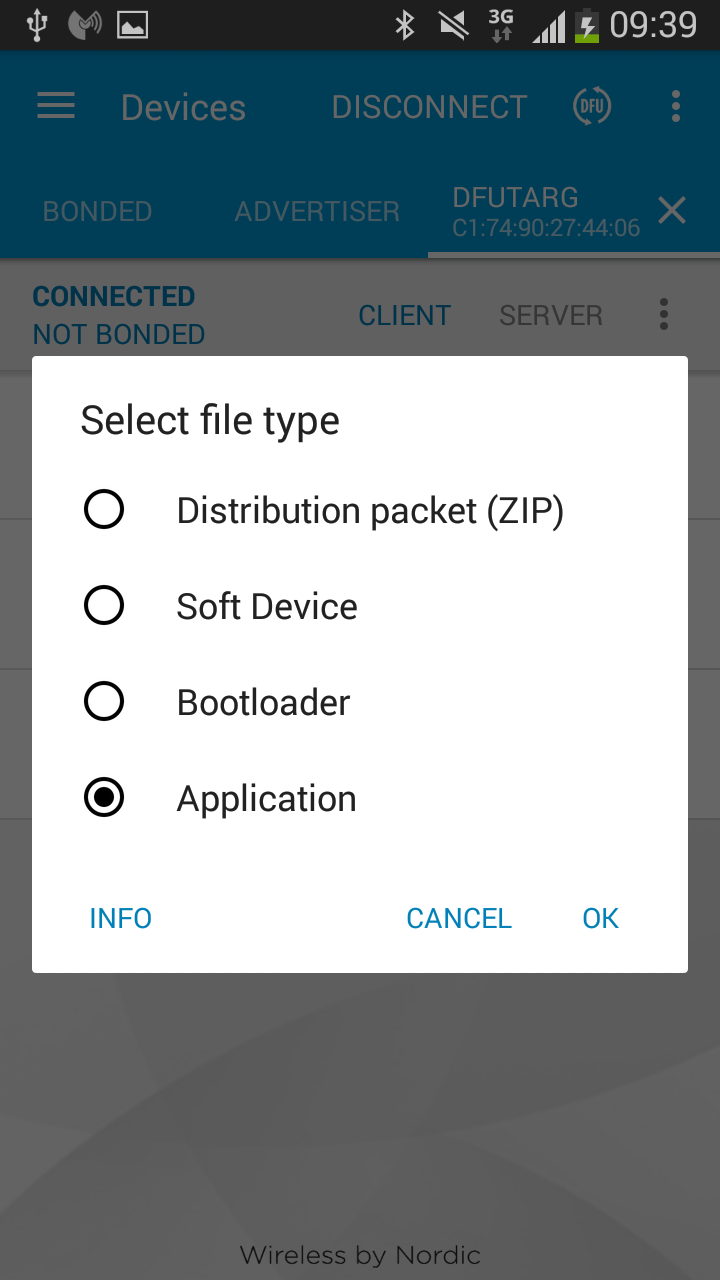
\includegraphics[scale=0.3]{FOTA6}
    \begin{minipage}{0.6\textwidth}
    \footnotesize
    \emph{File type select}
    \end{minipage}
\end{center}        

Zoek op het mobiele device naar de gecompileerde .hex file. Selecteer de .hex file. Na het selecteren van de .hex file, zal de service vragen of er een Init Packet nodig is voor het programmeren naar de Totem Health Patch. Let op: de *.bat file is niet nodig met de huidige firmware(S110 nRF51822 7.0.0). Selecteer 'NO' om verder te gaan met het uploaden van de firmware. 

\begin{center}
    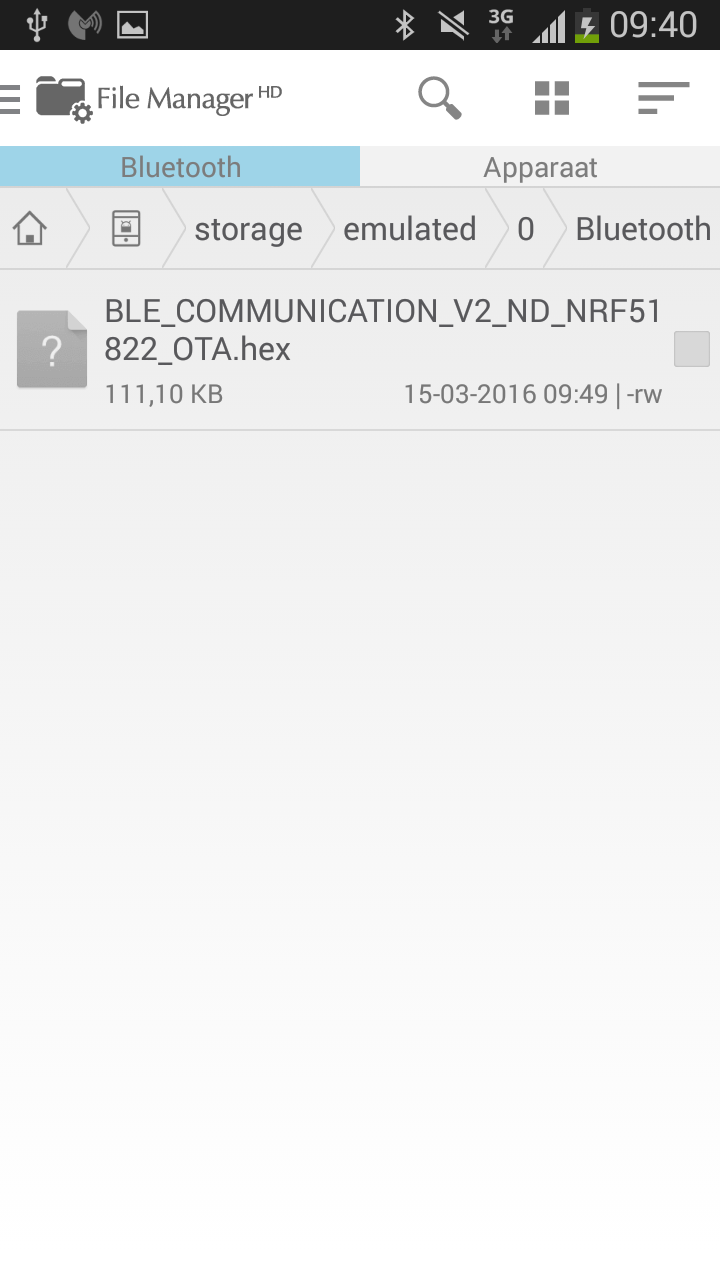
\includegraphics[scale=0.3]{FOTA7}
    \begin{minipage}{0.6\textwidth}
    \footnotesize
    \emph{File select}
    \end{minipage}
\end{center}

\begin{center}
    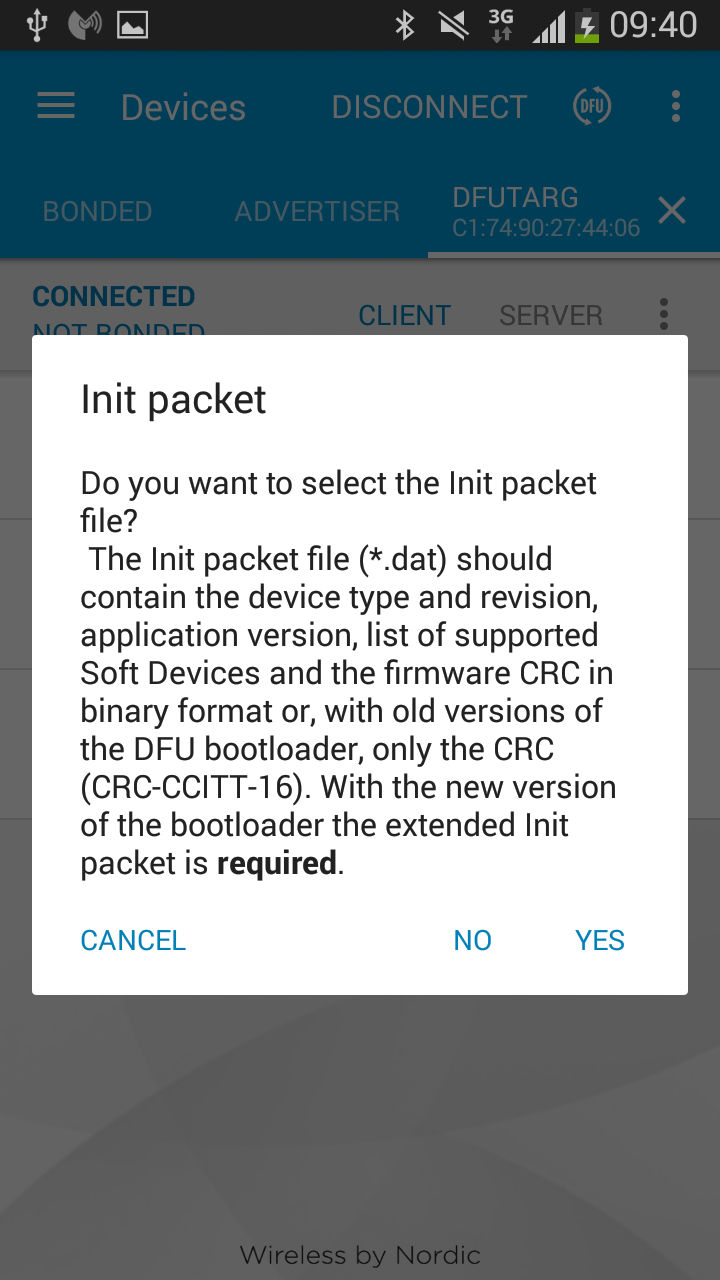
\includegraphics[scale=0.3]{FOTA8}
    \begin{minipage}{0.6\textwidth}
    \footnotesize
    \emph{Init packet}
    \end{minipage}
\end{center}

Op de onderstaande afbeelding is duidelijk zichtbaar dat het uploaden bijna klaar is.

\begin{center}
    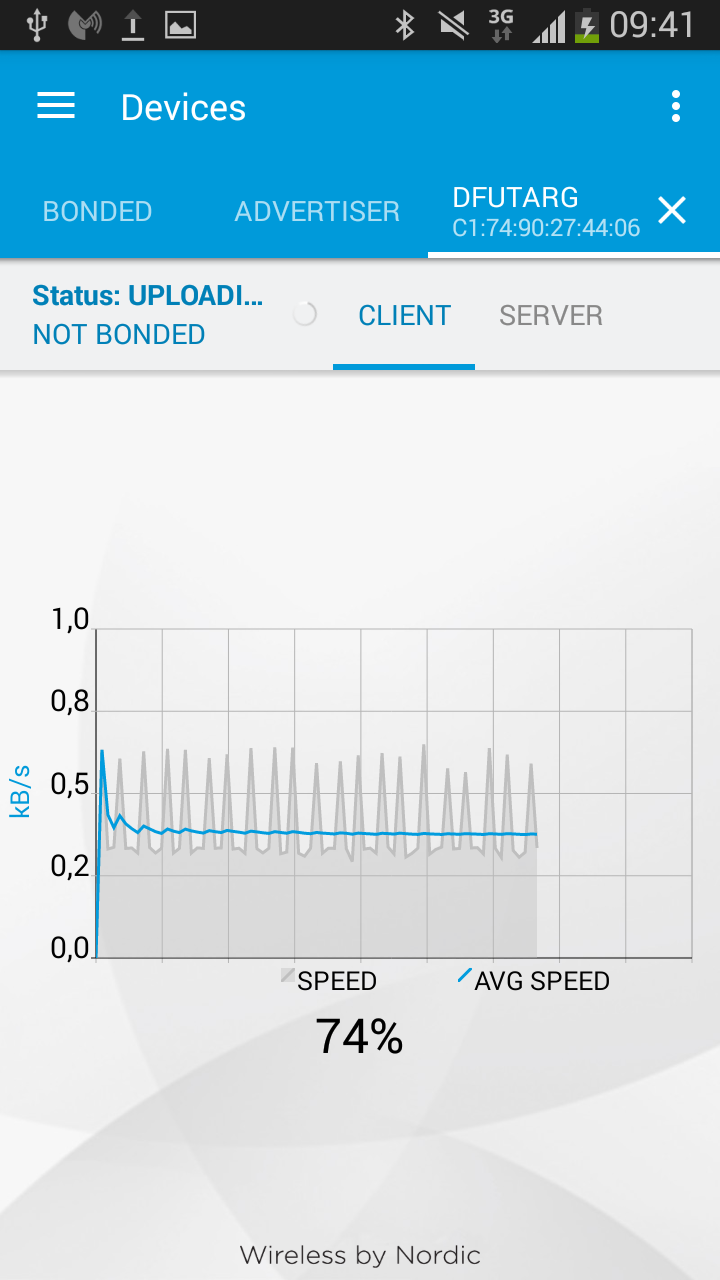
\includegraphics[scale=0.3]{FOTA9}
    \begin{minipage}{0.6\textwidth}
    \footnotesize
    \emph{Programming device}
    \end{minipage}
\end{center}
\newpage
De device discovery laat nu de geprogrammeerde Totem Health Patch zien.

\begin{center}
    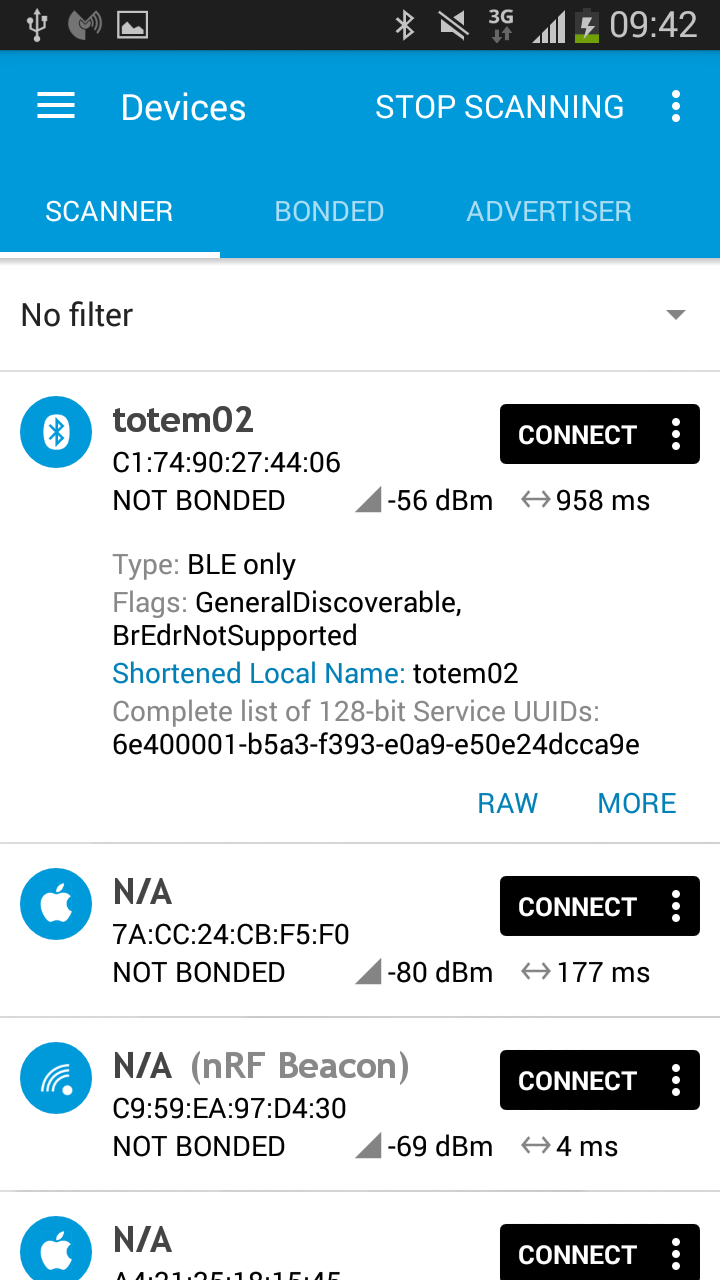
\includegraphics[scale=0.3]{FOTA10}
    \begin{minipage}{0.6\textwidth}
    \footnotesize
    \emph{Done}
    \end{minipage}
\end{center}

\section{Firmware Versie 1.0 en Device Applicatie}
Zoals aangegeven wordt er voor de open source Totem Health Patch software geschreven. Deze software staat online op de GitHub community. Hier vindt men de nieuwste voorbeelden en compleet werkende firmware versies die speciaal ontwikkeld zijn voor de Totem Open Source Health Patch. Bij de allernieuwste versie zit een android applicatie voor een realtime interface met de gebruiker. De android applicatie is te downloaden onder de volgende link.\\\\ \url{https://github.com/wemaketotem/TOTEM_HEALTH_PATCH_APK_REVISION1}\\\\ Sla de .apk file op, op een mobiel apparaat die Android als besturingssysteem heeft. Klik vervolgens op de .apk file om deze te installeren. Let op: het is noodzakelijk dat in de beveiligingsinstellingen van het mobiele apparaat, het installeren van derde partijen wordt toegestaan. Zie volgende afbeelding.

\begin{center}
    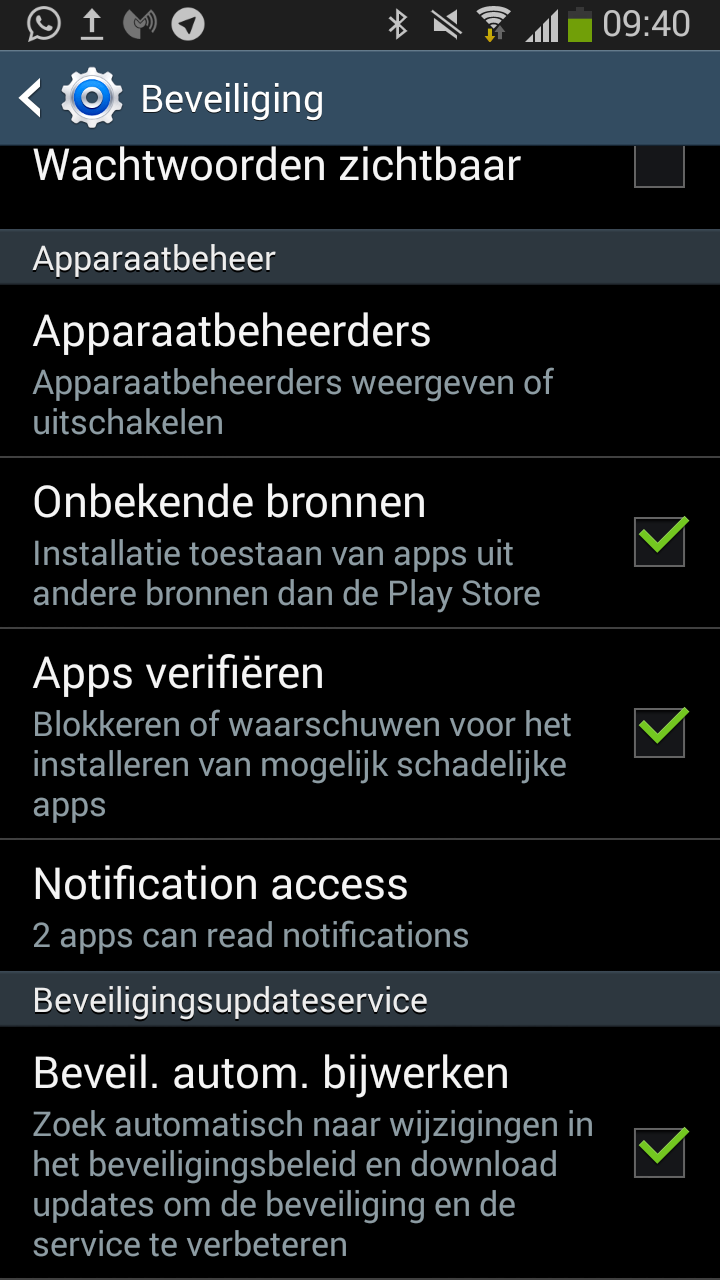
\includegraphics[scale=0.3]{thirdparty}
    \begin{minipage}{0.6\textwidth}
    \footnotesize
    \emph{Third party applicaties accepteren}
    \end{minipage}
\end{center}

Na het installeren van de applicatie kunt u met de applicatie zoeken naar actieve Totem apparaten. Wanneer de nieuwste firmware van de Totem Health Patch is geprogrammeerd, is de Health Patch vindbaar. De nieuwste firmware is te vinden onder de volgende link. \\\\\url{https://github.com/wemaketotem/TOTEM_HEALTH_PATCH_BLE_COMMUNICATION}\\\\De volgende afbeelding laat zien hoe de applicatie er moet uit zien wanneer deze juist is g"einstalleerd.

\begin{center}
    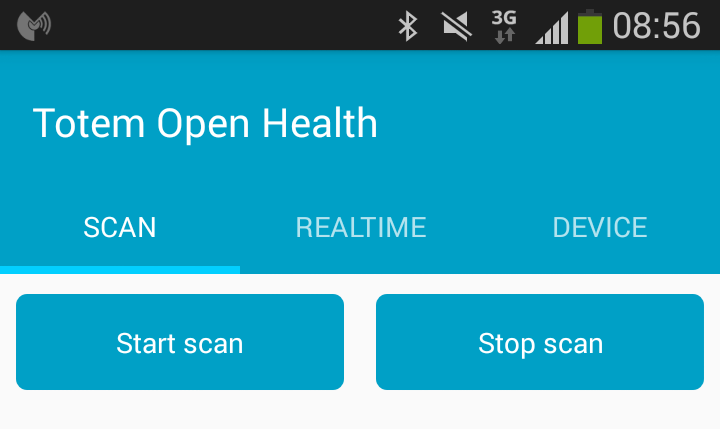
\includegraphics[scale=0.4]{apk1}
    \begin{minipage}{0.6\textwidth}
    \footnotesize
    \emph{Totem android applicatie apparaat zoeken}
    \end{minipage}
\end{center}

Als de Totem Health Patch is gevonden door de applicatie, kan er verbinding worden gemaakt. Door op het gevonden apparaat te drukken, wordt het snelmenu gestart en kan elke sensor individueel ingeschakeld of uitgeschakeld worden. \\\\In de nieuwste firmware zal het device 'totemX' genoemd worden. De bluetooth applicatie kan alleen Totem Health Patches vinden. Ieder ander apparaat is niet vindbaar door de device discovery. De applicatie maakt een melding wanneer Bluetooth niet is ingeschakeld. Er wordt toestemming gevraagd aan de gebruiker om Bluetooth in te schakelen. \\\\Wanneer de Health Patch is gevonden heeft het apparaat altijd de naam 'totemX'. De X staat voor een willekeurig nummer. Dit kan een getal zijn van 00 tot en met 99. Wanneer er zich meerdere Health Patches bevinden in dezelfde ruimte, moet het mogelijk zijn om de desbetreffende Health Patch te kunnen vinden. Zie afbeelding hieronder voor juiste zichtbaarheid van een Totem Health Patch. 

\begin{center}
    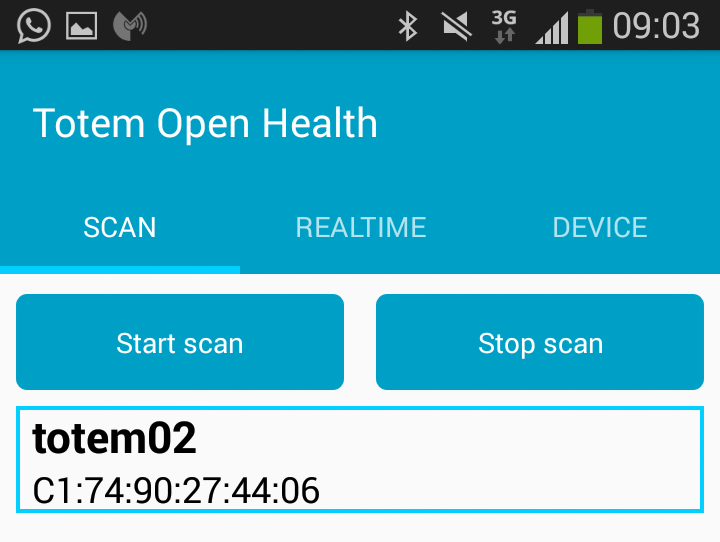
\includegraphics[scale=0.4]{apk2}
    \begin{minipage}{0.6\textwidth}
    \footnotesize
    \emph{Totem android applicatie apparaat zoeken}
    \end{minipage}
\end{center}

Let op: Na een positieve connectie is het belangrijk om enkele seconden te wachten. De Android applicatie heeft enkele seconden nodig om de Unix Timestamp te versturen. Tussen bovenstaande en onderstaande stappen is het belangrijk om de Health Patch te laten synchroniseren met de Android applicatie. 
 
\newpage
In het snelmenu worden de instellingen geconfigureerd. Elke sensor kan individueel worden ingeschakeld en uitgeschakeld. De knop 'Log Data' start een actuele meting. Let op: het is belangrijk dat er een SD kaart aanwezig is. Is dit niet het geval, dan kan de Health Patch geen data opslaan en zal de Health Patch niet vindbaar zijn door de applicatie. Het blauwe lampje zal gaan knipperen. De Health Patch zal wachten op een Sd kaart. De Health Patch gaat pas verder met het programma wanneer er een SD kaart wordt ingevoerd.\\\\Wanneer de meting actief is, kan de SD kaart niet worden verwijderd. Gebeurt dit wel dan is er naast een test.txt file geen data zichtbaar op de SD kaart. De Log data sessie moet worden afgesloten door de 'uit' knop. De sessie wordt afgesloten en de data wordt vastgelegd op de SD kaart. De SD kaart kan nu worden verwijderd en bekeken worden op een computer. Zie onderstaande afbeelding voor Totem Health Patch snelmenu. 
 
\begin{center}
    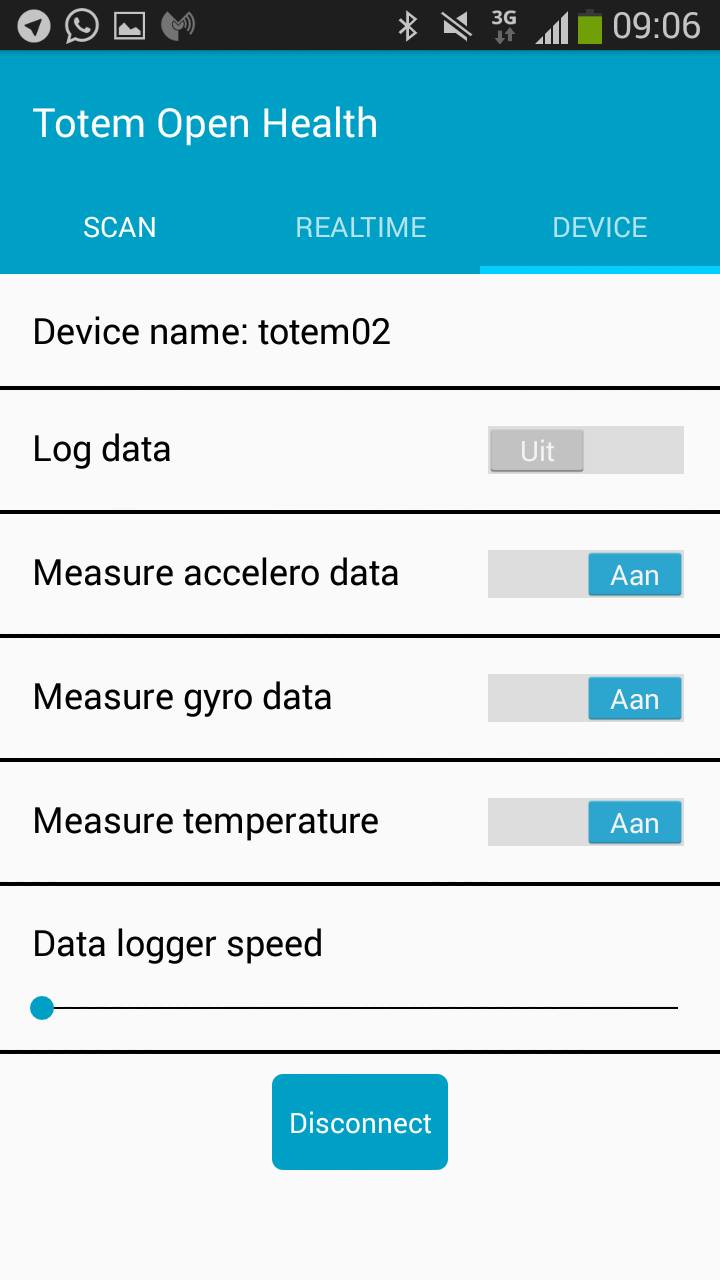
\includegraphics[scale=0.3]{apk3}
    \begin{minipage}{0.6\textwidth}
    \footnotesize
    \emph{Totem android applicatie snelmenu}
    \end{minipage}
\end{center}

De Totem Health Patch is nu klaar voor gebruik!

\begin{center}
    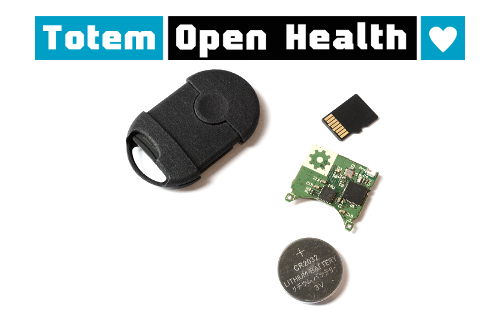
\includegraphics[scale=2.5]{totem}
    \begin{minipage}{0.6\textwidth}
    \footnotesize
    \emph{Totem Health Patch Kit}
    \end{minipage}
\end{center}

\end{document}